\documentclass{beamer}\usepackage[]{graphicx}\usepackage[]{color}
%% maxwidth is the original width if it is less than linewidth
%% otherwise use linewidth (to make sure the graphics do not exceed the margin)
\makeatletter
\def\maxwidth{ %
  \ifdim\Gin@nat@width>\linewidth
    \linewidth
  \else
    \Gin@nat@width
  \fi
}
\makeatother

\definecolor{fgcolor}{rgb}{0.345, 0.345, 0.345}
\newcommand{\hlnum}[1]{\textcolor[rgb]{0.686,0.059,0.569}{#1}}%
\newcommand{\hlstr}[1]{\textcolor[rgb]{0.192,0.494,0.8}{#1}}%
\newcommand{\hlcom}[1]{\textcolor[rgb]{0.678,0.584,0.686}{\textit{#1}}}%
\newcommand{\hlopt}[1]{\textcolor[rgb]{0,0,0}{#1}}%
\newcommand{\hlstd}[1]{\textcolor[rgb]{0.345,0.345,0.345}{#1}}%
\newcommand{\hlkwa}[1]{\textcolor[rgb]{0.161,0.373,0.58}{\textbf{#1}}}%
\newcommand{\hlkwb}[1]{\textcolor[rgb]{0.69,0.353,0.396}{#1}}%
\newcommand{\hlkwc}[1]{\textcolor[rgb]{0.333,0.667,0.333}{#1}}%
\newcommand{\hlkwd}[1]{\textcolor[rgb]{0.737,0.353,0.396}{\textbf{#1}}}%

\usepackage{framed}
\makeatletter
\newenvironment{kframe}{%
 \def\at@end@of@kframe{}%
 \ifinner\ifhmode%
  \def\at@end@of@kframe{\end{minipage}}%
  \begin{minipage}{\columnwidth}%
 \fi\fi%
 \def\FrameCommand##1{\hskip\@totalleftmargin \hskip-\fboxsep
 \colorbox{shadecolor}{##1}\hskip-\fboxsep
     % There is no \\@totalrightmargin, so:
     \hskip-\linewidth \hskip-\@totalleftmargin \hskip\columnwidth}%
 \MakeFramed {\advance\hsize-\width
   \@totalleftmargin\z@ \linewidth\hsize
   \@setminipage}}%
 {\par\unskip\endMakeFramed%
 \at@end@of@kframe}
\makeatother

\definecolor{shadecolor}{rgb}{.97, .97, .97}
\definecolor{messagecolor}{rgb}{0, 0, 0}
\definecolor{warningcolor}{rgb}{1, 0, 1}
\definecolor{errorcolor}{rgb}{1, 0, 0}
\newenvironment{knitrout}{}{} % an empty environment to be redefined in TeX

\usepackage{alltt} 
% \usepackage{graphicx}
\usepackage{graphics}
\usepackage[T1]{fontenc}
\usepackage{hyperref}
\setbeamercovered{transparent}
\renewcommand{\ni}{\noindent}
\hypersetup{
  colorlinks   = true, %Colours links instead of ugly boxes
  urlcolor     = blue, %Colour for external hyperlinks
  linkcolor    = blue, %Colour of internal links
  citecolor   = red %Colour of citations
}
%% to include page numbers manually include the next three lines
% \usepackage{fancyhdr,lastpage}
% \pagestyle{fancy}\fancyhf{}\rfoot{\vspace{-0.5cm} Page {\thepage} of \pageref{LastPage}}
% \renewcommand\headrulewidth{0pt} % Removes funny header line
%load packages that will be invisible on slides



\title[Advanced Graphics in R ]{2 - Advanded Graphics in R}
\subtitle{01 - Basic Plots}
\date{\hspace{1in}}
\institute[ISU]{Iowa State University}
\IfFileExists{upquote.sty}{\usepackage{upquote}}{}
\begin{document}

\begin{frame}
    \maketitle
\end{frame}

%---------------------------------------------------------------------------

\begin{frame}
\frametitle{ggplot2 in a nutshell}
    \begin{itemize}
        \item Package for statistical graphics
        \item Developed by Hadley Wickham (An ISU Alumni)
        \item Designed to adhere to good graphical practices
        \item Supports a wide variety plot types
        \item Constructs plots using the concept of layers\medskip
        \item \url{http://had.co.nz/ggplot2/} or Hadley's book \begin{center}\emph{ggplot2: Elegant Graphics for Data Analysis}\end{center} for reference material
    \end{itemize}    
\end{frame}

%---------------------------------------------------------------------------

\begin{frame}
\frametitle{\texttt{qplot()}}
  \texttt{qplot()} function is the basic workhorse of ggplot2\bigskip
    \begin{itemize}
        \item produces all plot types available with ggplot2\medskip
        \item allows for plotting options within the function statement\medskip
        \item creates an object that can be saved\medskip
        \item plot layers can be added to modify plot complexity
    \end{itemize}    
\end{frame}

%---------------------------------------------------------------------------

\begin{frame}
\frametitle{\texttt{qplot()} structure}
  \texttt{qplot()} function has a basic syntax

\vspace{.1in}

\begin{center}
\texttt{qplot(variables, plot type, dataset, options)}
\end{center}

\begin{itemize}
  \item variables: list of variables used for the plot\medskip
  \item plot type: specified with a \texttt{geom=} statement\medskip
  \item dataset: specified with a \texttt{data=} statement\medskip
  \item options: there are so, so many options!
\end{itemize}

\end{frame}

%---------------------------------------------------------------------------

\begin{frame}
\frametitle{Diamonds Data}

We will explore the diamonds data set (preloaded along with ggplot2) using qplot for basic plotting.\\
\bigskip

The data set was scraped from a diamond exchange company data base by Hadley.  It contains the prices and attributes of over 50,000 diamonds

\end{frame}

%---------------------------------------------------------------------------

\begin{frame}[fragile]
\frametitle{Examining the Diamonds Data}
    
What does the data look like?\bigskip

Lets look at the top few rows of the diamond data frame to find out!
    
\footnotesize
\begin{knitrout}\scriptsize
\definecolor{shadecolor}{rgb}{1, 1, 1}\color{fgcolor}\begin{kframe}
\begin{alltt}
\hlkwd{head}\hlstd{(diamonds)}
\end{alltt}
\begin{verbatim}
##   carat       cut color clarity depth table price    x    y    z
## 1  0.23     Ideal     E     SI2  61.5    55   326 3.95 3.98 2.43
## 2  0.21   Premium     E     SI1  59.8    61   326 3.89 3.84 2.31
## 3  0.23      Good     E     VS1  56.9    65   327 4.05 4.07 2.31
## 4  0.29   Premium     I     VS2  62.4    58   334 4.20 4.23 2.63
## 5  0.31      Good     J     SI2  63.3    58   335 4.34 4.35 2.75
## 6  0.24 Very Good     J    VVS2  62.8    57   336 3.94 3.96 2.48
\end{verbatim}
\end{kframe}
\end{knitrout}
\normalsize
\end{frame}

%---------------------------------------------------------------------------

\begin{frame}
\frametitle{\texttt{qplot()} demo}

   Demo of basic plot types and options using \texttt{qplot()}!
   
   \vspace{.2in}
   
   Follow along with the demo by opening GraphicsIntro.R in your own R environment

\end{frame}

%---------------------------------------------------------------------------

\begin{frame}[fragile]
\frametitle{Scatterplot}
    
    Basic scatter plot of diamond price vs carat weight
    
\footnotesize
\begin{knitrout}\footnotesize
\definecolor{shadecolor}{rgb}{1, 1, 1}\color{fgcolor}\begin{kframe}
\begin{alltt}
\hlkwd{qplot}\hlstd{(carat, price,} \hlkwc{geom}\hlstd{=}\hlstr{"point"}\hlstd{,} \hlkwc{data}\hlstd{=diamonds)}
\end{alltt}
\end{kframe}

{\centering 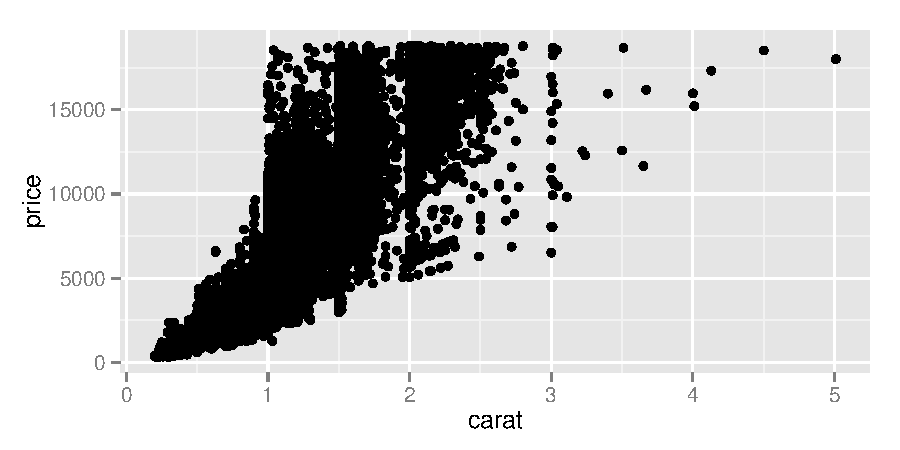
\includegraphics[width=.9\linewidth]{figure/kdiamondscatter1} 

}



\end{knitrout}
\normalsize
\end{frame}

%---------------------------------------------------------------------------

\begin{frame}[fragile]
\frametitle{Scatterplot}
    
    Scatter plot of diamond price vs carat weight showing versitility of options in qplot
    
\footnotesize
\begin{knitrout}\footnotesize
\definecolor{shadecolor}{rgb}{1, 1, 1}\color{fgcolor}\begin{kframe}
\begin{alltt}
\hlkwd{qplot}\hlstd{(carat,} \hlkwd{log}\hlstd{(price),} \hlkwc{geom}\hlstd{=}\hlstr{"point"}\hlstd{,} \hlkwc{data}\hlstd{=diamonds,}
        \hlkwc{alpha}\hlstd{=}\hlkwd{I}\hlstd{(}\hlnum{.2}\hlstd{),} \hlkwc{colour}\hlstd{=color,}
        \hlkwc{main}\hlstd{=}\hlstr{"Log price by carat weight, grouped by color"}\hlstd{)}
\end{alltt}
\end{kframe}

{\centering 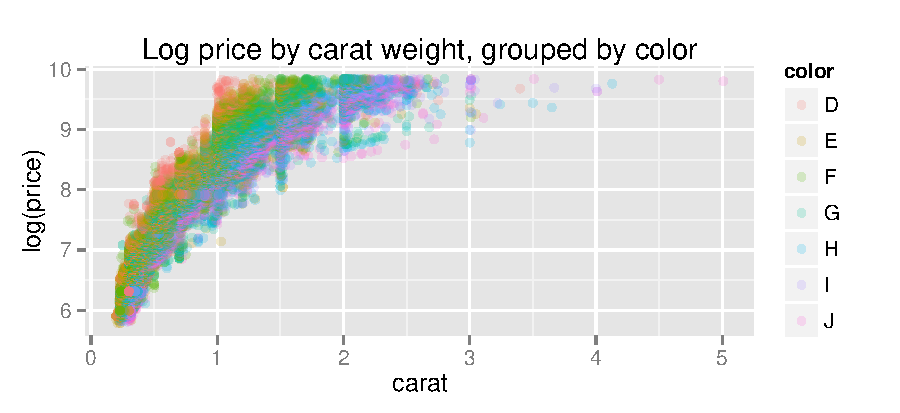
\includegraphics[width=.9\linewidth]{figure/kdiamondscatter2} 

}



\end{knitrout}
\normalsize
\end{frame}

%---------------------------------------------------------------------------

\begin{frame}
\frametitle{Your Turn}

All of the your turns for this section will use the tips data set (loaded in with reshape package)
  
\begin{knitrout}\footnotesize
\definecolor{shadecolor}{rgb}{1, 1, 1}\color{fgcolor}\begin{kframe}
\begin{alltt}
\hlkwd{data}\hlstd{(tips,} \hlkwc{package}\hlstd{=}\hlstr{"reshape2"}\hlstd{)}
\end{alltt}
\end{kframe}
\end{knitrout}

\begin{itemize}
  \item Use qplot to build a scatterplot of variables tips and total bill\medskip
  \item Use options within qplot to color points by smokers\medskip
  \item Clean up axis labels and add main plot title\medskip
\end{itemize}

\end{frame}


%---------------------------------------------------------------------------

\begin{frame}[fragile]
\frametitle{Histograms}
    
Basic histogram of carat weight
    
\footnotesize
\begin{knitrout}\footnotesize
\definecolor{shadecolor}{rgb}{1, 1, 1}\color{fgcolor}\begin{kframe}
\begin{alltt}
\hlkwd{qplot}\hlstd{(carat,} \hlkwc{geom}\hlstd{=}\hlstr{"histogram"}\hlstd{,} \hlkwc{data}\hlstd{=diamonds)}
\end{alltt}


{\ttfamily\noindent\itshape\color{messagecolor}{\#\# stat\_bin: binwidth defaulted to range/30. Use 'binwidth = x' to adjust this.}}\end{kframe}

{\centering 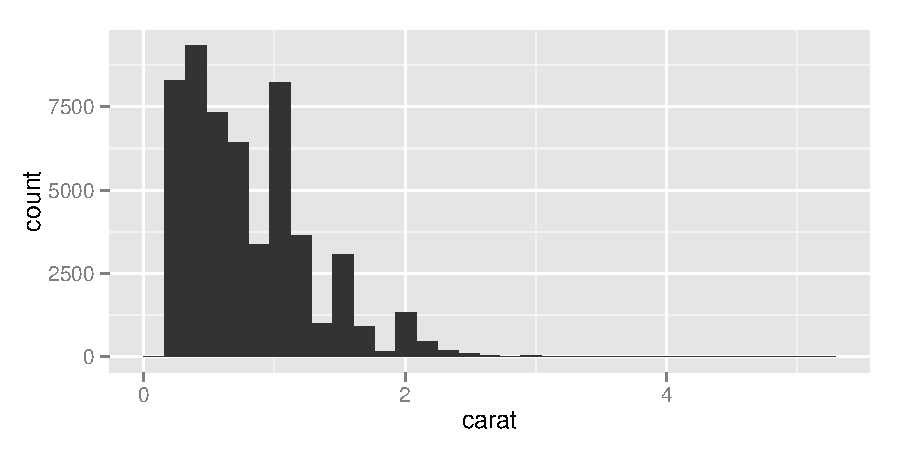
\includegraphics[width=.9\linewidth]{figure/kdiamondhist1} 

}



\end{knitrout}
\normalsize
\end{frame}



%---------------------------------------------------------------------------

\begin{frame}[fragile]
\frametitle{Histograms}
    
Carat weight histograms faceted by cut
    
\footnotesize
\begin{knitrout}\footnotesize
\definecolor{shadecolor}{rgb}{1, 1, 1}\color{fgcolor}\begin{kframe}
\begin{alltt}
\hlkwd{qplot}\hlstd{(carat,} \hlkwc{geom}\hlstd{=}\hlstr{"histogram"}\hlstd{,} \hlkwc{data}\hlstd{=diamonds,}
                        \hlkwc{binwidth}\hlstd{=}\hlnum{.2}\hlstd{,} \hlkwc{facets}\hlstd{=.}\hlopt{~}\hlstd{cut )}
\end{alltt}
\end{kframe}

{\centering 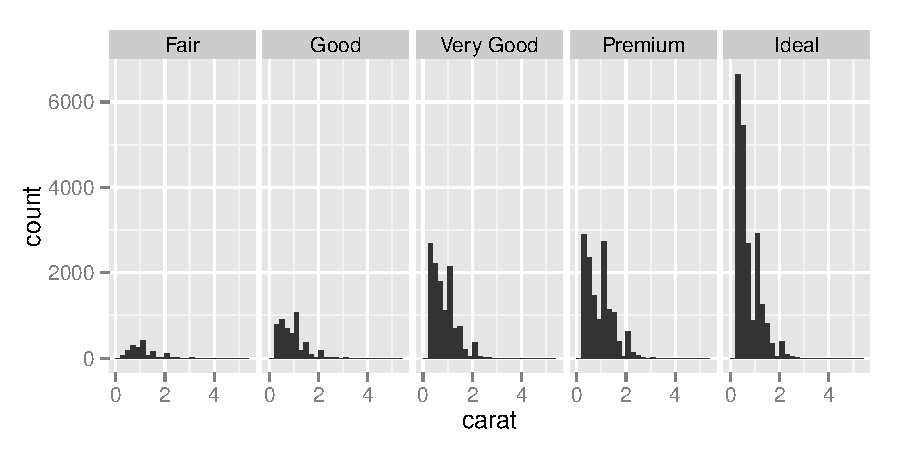
\includegraphics[width=.9\linewidth]{figure/kdiamondhist2} 

}



\end{knitrout}
\normalsize
\end{frame}

%---------------------------------------------------------------------------

\begin{frame}
\frametitle{Your Turn}

\begin{itemize}
  \item Create a new variable in tips data frame rate = tip/total bill\medskip
  \item Use qplot to create a histogram of rate\medskip
  \item Change the bin width on that histogram to 0.05\medskip
  \item Facet this histogram by size of the group
\end{itemize}

\end{frame}

%---------------------------------------------------------------------------

\begin{frame}[fragile]
\frametitle{Boxplots}
    
    Side by side boxplot of diamond prices within cut groupings
    
\footnotesize
\begin{knitrout}\footnotesize
\definecolor{shadecolor}{rgb}{1, 1, 1}\color{fgcolor}\begin{kframe}
\begin{alltt}
\hlkwd{qplot}\hlstd{(cut, price,} \hlkwc{geom}\hlstd{=}\hlstr{"boxplot"}\hlstd{,} \hlkwc{data}\hlstd{=diamonds)}
\end{alltt}
\end{kframe}

{\centering 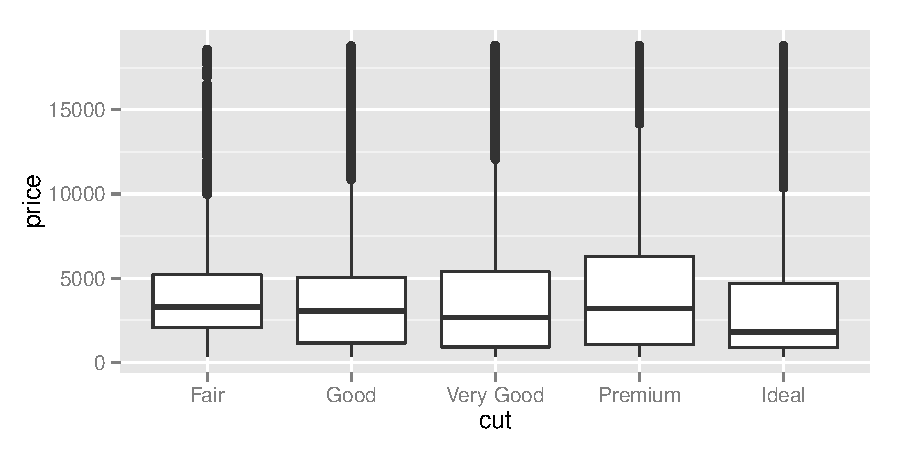
\includegraphics[width=.9\linewidth]{figure/kdiamondbox1} 

}



\end{knitrout}
\normalsize
\end{frame}

%---------------------------------------------------------------------------

\begin{frame}[fragile]
\frametitle{Boxplots}
    
    Side by side boxplot of log prices within cut groupings with jittered values overlay
    
\footnotesize
\begin{knitrout}\scriptsize
\definecolor{shadecolor}{rgb}{1, 1, 1}\color{fgcolor}\begin{kframe}
\begin{alltt}
\hlkwd{qplot}\hlstd{(cut,} \hlkwd{log}\hlstd{(price),} \hlkwc{geom}\hlstd{=}\hlstr{"boxplot"}\hlstd{,} \hlkwc{data}\hlstd{=diamonds,}
        \hlkwc{main}\hlstd{=}\hlstr{"Boxplots of log Diamond Prices Grouped by Cut Quality"}\hlstd{)} \hlopt{+}
        \hlkwd{geom_jitter}\hlstd{(}\hlkwc{alpha}\hlstd{=}\hlkwd{I}\hlstd{(}\hlnum{.025}\hlstd{))}
\end{alltt}
\end{kframe}

{\centering 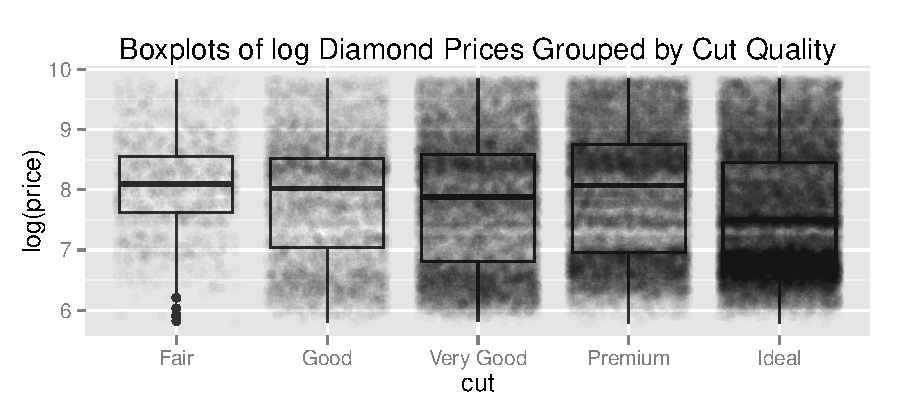
\includegraphics[width=.9\linewidth]{figure/kdiamondbox2} 

}



\end{knitrout}
\normalsize
\end{frame}

%---------------------------------------------------------------------------

\begin{frame}
\frametitle{Your Turn}

\begin{itemize}
  \item Make side by side boxplots of tipping rate for males and females\medskip
  \item Overlay jittered points for observed values onto this boxplot
\end{itemize}

\end{frame}

%---------------------------------------------------------------------------

\begin{frame}
\frametitle{Bar plots}
    
To investigate bar plots we will switch over to the Titanic data set
\begin{knitrout}\footnotesize
\definecolor{shadecolor}{rgb}{1, 1, 1}\color{fgcolor}\begin{kframe}
\begin{alltt}
\hlstd{titanic} \hlkwb{<-} \hlkwd{as.data.frame}\hlstd{(Titanic)}
\end{alltt}
\end{kframe}
\end{knitrout}
\bigskip
    
Data includes passenger characteristics and survival outcomes for those aboard the RMS Titanics ill fated maiden voyage
    
\end{frame}

%---------------------------------------------------------------------------

\begin{frame}[fragile]
\frametitle{Bar Plots}
    
Basic bar plot of survival outcomes
    
\footnotesize
\begin{knitrout}\footnotesize
\definecolor{shadecolor}{rgb}{1, 1, 1}\color{fgcolor}\begin{kframe}
\begin{alltt}
\hlkwd{qplot}\hlstd{(Survived,} \hlkwc{geom}\hlstd{=}\hlstr{"bar"}\hlstd{,} \hlkwc{data}\hlstd{=titanic,} \hlkwc{weight}\hlstd{=Freq)}
\end{alltt}
\end{kframe}

{\centering 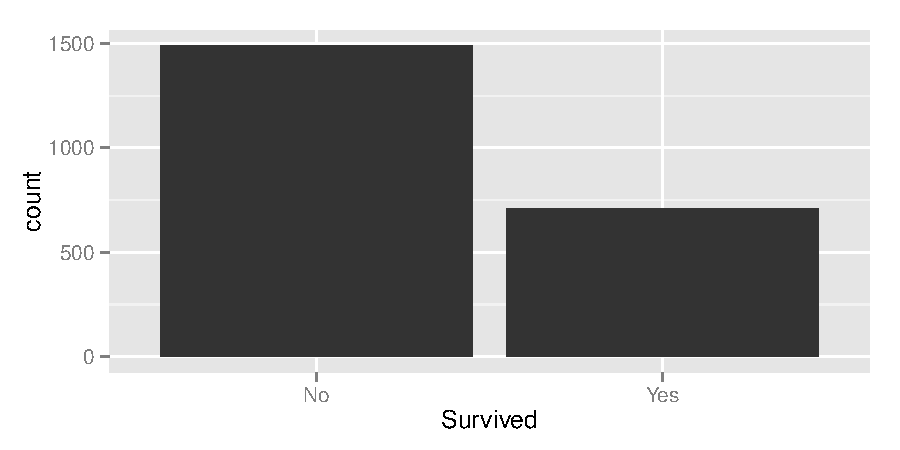
\includegraphics[width=.9\linewidth]{figure/kdiamondbar1} 

}



\end{knitrout}
\normalsize
\end{frame}

%---------------------------------------------------------------------------

\begin{frame}[fragile]
\frametitle{Bar Plots}
    
Bar plot faceted by gender and class
    
\footnotesize
\begin{knitrout}\footnotesize
\definecolor{shadecolor}{rgb}{1, 1, 1}\color{fgcolor}\begin{kframe}
\begin{alltt}
\hlkwd{qplot}\hlstd{(Survived,} \hlkwc{geom}\hlstd{=}\hlstr{"bar"}\hlstd{,} \hlkwc{data}\hlstd{=titanic,}
                        \hlkwc{weight}\hlstd{=Freq,} \hlkwc{facets}\hlstd{=Sex}\hlopt{~}\hlstd{Class)}
\end{alltt}
\end{kframe}

{\centering 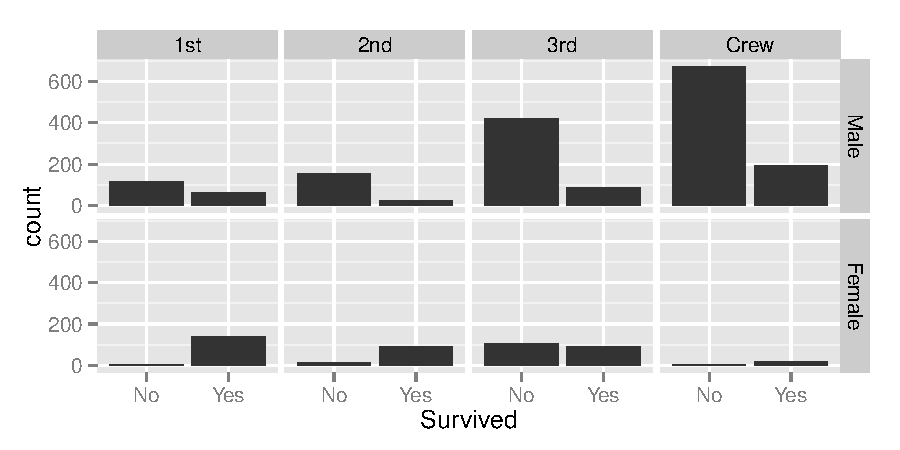
\includegraphics[width=.9\linewidth]{figure/kdiamondbar2} 

}



\end{knitrout}
\normalsize
\end{frame}


%---------------------------------------------------------------------------

\begin{frame}
\frametitle{Your Turn}

\begin{itemize}
  \item Use the tips data to make a barplot for counts of smoking and non smoking customers\medskip
  \item Facet using day of week and time of day to view how smoking status changes for different meal times
\end{itemize}

\end{frame}

\end{document}
